\chapter{Implementation details}\label{ch:implementation}

This specifies the implementation details of the project, that is, the most significant aspects regarding the coding of the system and its functionalities.

The description of this issues aims at easing possible future enhancements of the system and the maintenance of the code. Some specific aspects of the programming of the code are described and some of the choices made during the implementation process are justified.

\section{Coding style}

There are several well known coding patterns for JavaScript programs. In this project the Google JavaScript Style Guide \cite{googlestyle} has been followed. Below some of the relevant guidelines, and the reasons behind them are listed.

\begin{itemize}
\item Always use \texttt{var} for variable declarations. This is done to avoid the runtime placing the variable in the global context, which can cause overriding of other variables.
\item Variables and functions are named in camelCase, that is, any multi-word name will be written as a single word with the first letter of every additional word in uppercase.
\item Always use semicolons. JS runtimes can run code without the semicolons, however, in some cases they may cause subtle hard to debug errors.
\item Use \texttt{foo.bar = null;} to delete. This is done because the \texttt{delete} operator in JS is slower on many runtime environments. 
\item Use single quotes instead of double quotes. This is a standard across most JS coding styles, for it makes easier to write XML and HTML string, a common task.
\end{itemize}

This are some of the most common guidelines followed, however, there are more rules and small tricks followed, such as caching the array lengths in loops.

\section{Development environment}

This section describes the tools used on the development process. This tools are directly related to the development process but not to the final product.

\subsection{Atom text editor}

Atom is a JavaScript coding oriented configurable text editor developed by GitHub \cite{atom}. It is available for all major operating systems, however it only has prebuilt packages for OS X. Anyway, it provides a repository for Ubuntu OSs which has been used to install it.

The editor is very similar to Sublime Text 2 \cite{sublime} and while Sublime has more years of development and a bigger community behind, Atom offers native NodeJS and Git integration, which declines the balance in favor of Atom for this project. 

It has been used on the project as the sole code editor. An overview of the interface it offers is shown in figure \ref{fig:atom}.

\begin{figure}[ht]
  \centering
  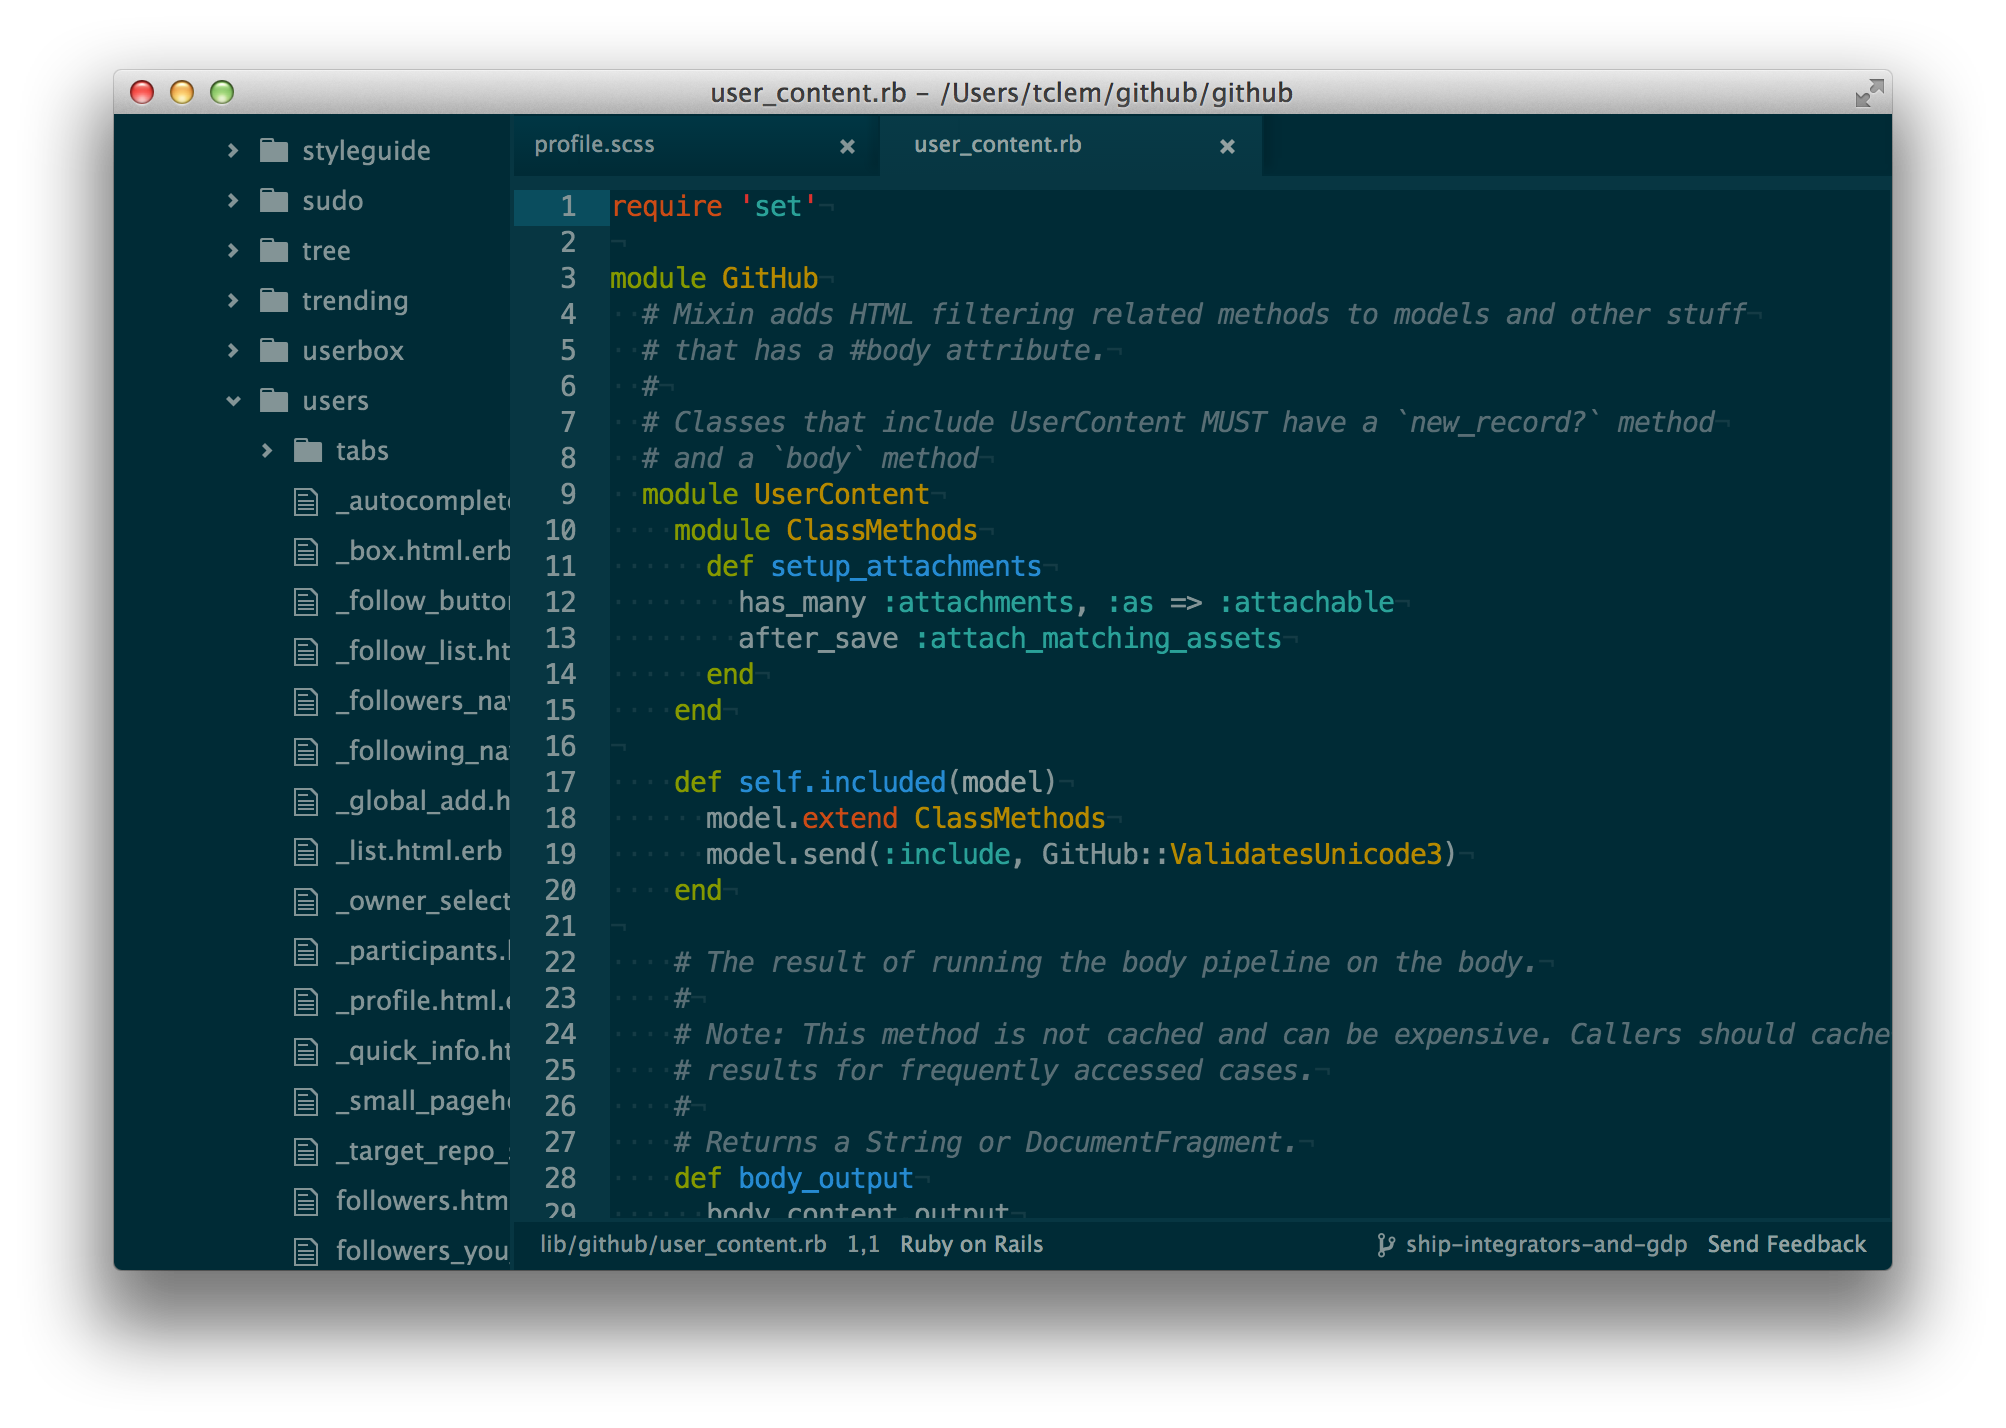
\includegraphics[width=.8\textwidth]{fig/atom}
  \caption{The Atom text editor}
  \captionsetup{font={footnotesize,bf,it}}
  \label{fig:atom}
\end{figure} 

\subsection{Git}

Git \cite{git} is a free and open source distributed version control system with emphasis on speed. 

It has been a very popular tool on open source projects ever since it was developed by Linus Torvalds. It supports the classic functionalities found on all version control systems, in addition to several additional functionalities which make it a superior choice.

The main advantage of GIT is being distributed. Thanks to this it is possible to have local repositories in different machines and synchronize all of them on a single repository, having each local repository keep copies of the whole project.

This project is hosted in the GitHub platform, a free open source project hosting site which supports GIT. A student account, providing three private repositories has been provided by the organization itself.

\subsection{Yeoman}

Yeoman \cite{yo} is a generator ecosystem that helps kickstarting new projects by prescribing best practices and productive tools. 

This tool acts as a command line interface that scaffolds projects, that is, it automatically builds project skeletons which incorporate modern tools. It is based on generators, which specify how an project is created and which technologies are to be used in it.

The development team of Yeoman has created a series of official generators, however, there are several community defined generators that can be used to scaffold different types of projects. This project has used the angular-fullstack generator, used to scaffold a express application which uses AngularJS on the client side.

\subsection{Grunt}

Grunt \cite{grunt} is a JavaScript automation tool that allow to run tasks such as compilation, testing and minification. It becomes incorporated in the majority of the yeoman generators and it is very useful for the deployment tasks of a project, such as code minification and compilation to JavaScript.

It has been used to run the testing, serving and building processes of the project.

\subsection{JSLint}

JSLint \cite{jslint} is a static code analysis tool that promotes and tries to enforce code quality on JavaScript. It works by ensuring that the source code on JavaScript application follows coding rules and best practices.

Grunt can be used to automate the running of JSLint on code changes. In this project, all the source code has been checked using this tool, and no code has been deployed without passing a linter with no errors.

\subsection{Prot\'eg\'e-OWL}

Prot\'eg\'e is an open-source ontology editor and framework for building intelligent systems\cite{protege1}. The traditional architecture of the editor is based on frames \cite{protege2}, however, with the standardization of OWL (see section \ref{sec:owl}) support for this language was added to the framework \cite{protege3}.

The current version of Prot\'eg\'e can be used to edit classes and their characteristics, to access different reasoning engines, to edit and execute queries and rules and to visualize relationships between concepts. The tool has been widely adopted by the Semantic Web ontologists, for all their utilities and because it has been adopted among the W3C recommendations \cite{protege4}.

The tool provides a graphical user interface, which can be seen in figure \ref{fig:protege}. Through this editor, other vocabularies can be imported, in addition to create classes and properties for a new ontology and defining restrictions and relations among them. It has been used to create the SORELCOM ontology on the project.

\begin{figure}[ht]
  \centering
  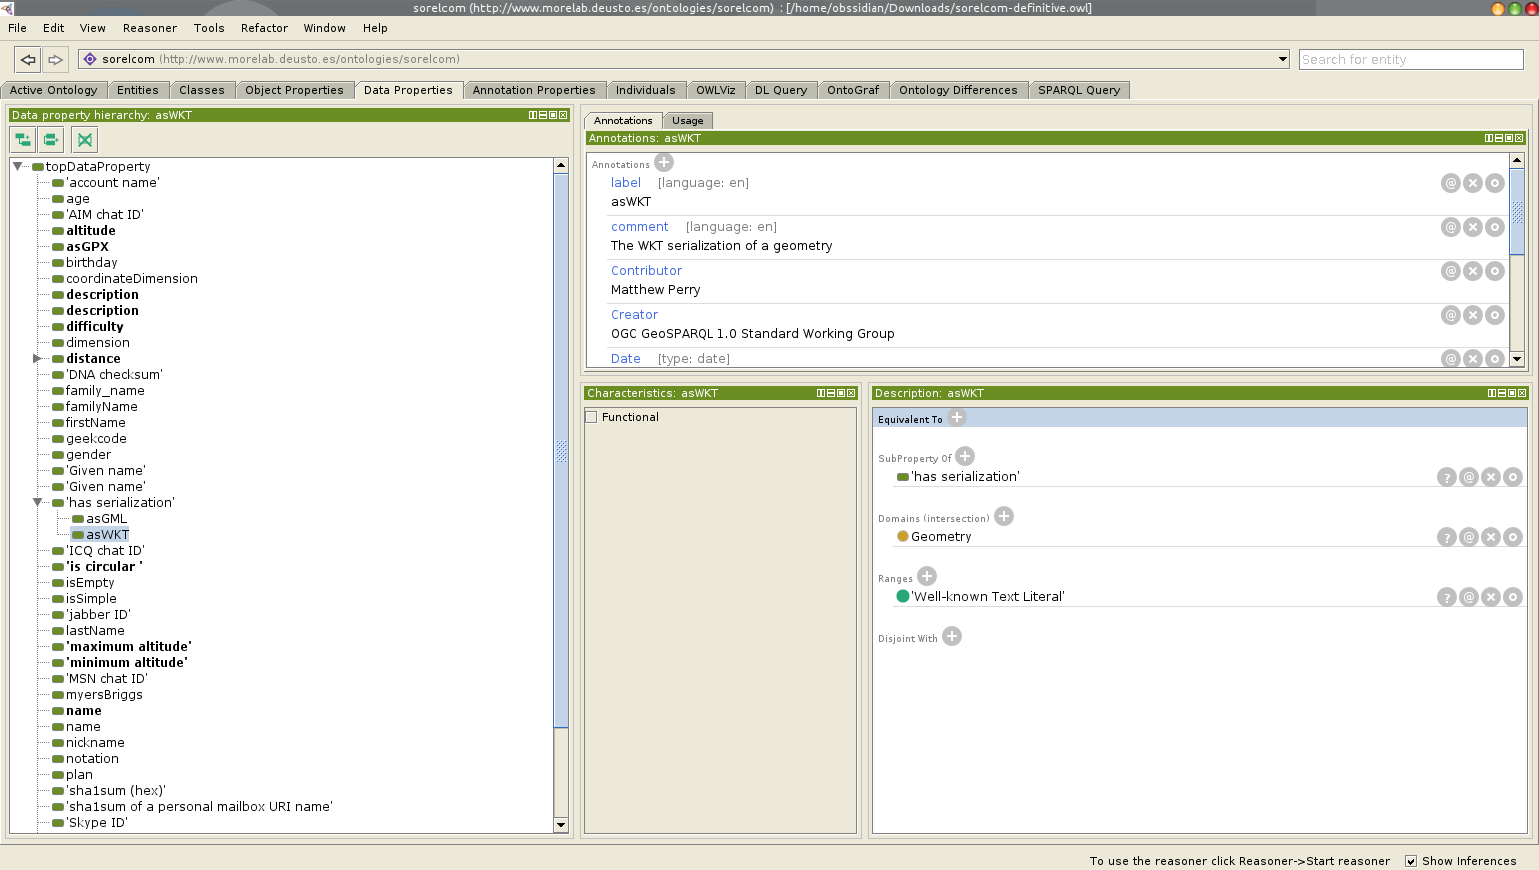
\includegraphics[width=.8\textwidth]{fig/protege}
  \caption{The Prot\'eg\'e OWL ontology editor}
  \captionsetup{font={footnotesize,bf,it}}
  \label{fig:protege}
\end{figure} 

\section{Development of the server}\label{sec:serverdev}

The first step, after the technology research and the design consideration for the development of the project has been the creation of a project using the Yeoman tool. Even though initially only the server is developed, the project skeleton contains a section for the web application, for convenience purposes.

The generator used is the angular-fullstack generator, hosted on \href{https://github.com/DaftMonk/generator-angular-fullstack} and offered though the \textit{generator-angular-fullstack} npm package. 

This command creates the following folder structure.

\begin{description}
\item[app] Contains the code for the web application. Its structure is detailed in section \ref{sec:webappdev}.
\item[lib] Contains the code for the web server.
\item[test] Contains the tests to be run.
\item[node\_modules] Contains the libraries used in the server. It is a mandatory folder in any NodeJS application.
\item [dist] This folder does not exist initially, however, after running the build task it will be populated with the distributable code.
\end{description}

\subsection{NodeJS application structure}

All the code for the server is found inside the \textit{lib} folder. There is still no consensus by the community on which is the file structure that this kind of servers should follow, thus the following structure has been used.

\begin{description}
\item[utils] Utility classes, such as the geographic analyser.
\item[connector] Classes related to the database connector
\item[controllers] Controllers of the server
\item[models] Models of the server 
\item[\textit{routes.js}] Specification of the URLs that the server will route. It is a file, not a folder. 
\end{description}

\subsubsection*{Modules}

External libraries, modules, are used in the Node projects through the keyword \textit{require}. When a module is downloaded through the NPM package manager it is stored in the \textit{node\_modules} folder and can be referenced by a previously defined name. An example of this can be found in listing \ref{lst:require}

\begin{listing}[ht]\centering
  \begin{minipage}{.6\textwidth}
    \begin{minted}[linenos=true,mathescape,gobble=6]{js}
         /** A module called requests is required, an will later be used
         by referencing the variable where it is stored. */
	     var requests = require('requests');
    \end{minted}
  \end{minipage}
  \caption{NodeJS module requiring}\label{lst:require}
\end{listing}

In order to use code defined on files different from the main server, the same mechanism is used. The \textit{require} command obtains an object after running the code on the specified module. The object obtained through the require command is called \texttt{module.exports}. This object is just a dictionary where the function, objects or classes to be exported are appended.

\subsection{Semantic database}

For the server to be able to implement its functionality, it is necessary to first install the database. The storage system to be used is named Parliament, it includes a triple store, a reasoner that supports OWL and GeoSPARQL and a HTTP SPARQL endpoint. 

Two types of packages are offered, which can be found in \href{http://semwebcentral.org/frs/?group_id=159}, the QuickStart bundles and the source files. In this project, a QuickStart bundle for a Linux environment has been used. The advantage of this is that there is no need to install any file to the machine, everything is provided and the database can be running by executing the \textit{StartParliament.sh} file provided.

This bundle uses Jetty, a Java based HTTP server, \textit{jetty.xml} file provided. The default configuration is usually enough, however, since large SPARQL queries are to be done, the form submission size has been changed. The element in listing \ref{lst:jetty} has been added in order to allow the upload of large trails.

\begin{listing}[ht]\centering
  \begin{minipage}{.6\textwidth}
    \begin{minted}[linenos=true,mathescape,gobble=6]{xml}
	     <Call class="java.lang.System" name="setProperty">
	        <Arg>org.mortbay.jetty.Request.maxFormContentSize</Arg>
	        <Arg>500000</Arg>
	     </Call>
    \end{minted}
  \end{minipage}
  \caption{Jetty server configuration}\label{lst:jetty}
\end{listing}

Once the server is configured and running, it can be accessed on the port 8080, using the URL \texttt{http://localhost:8080/parliament}. Doing so offers a interface for the administration and exploration of the triple store. The final step for the installation of the database is configuring the RDF graph on which the information will be saved to generate spatial indexes, which can be done from this interface, as shown in figure \ref{fig:parliament}

\begin{figure}[ht]
  \centering
  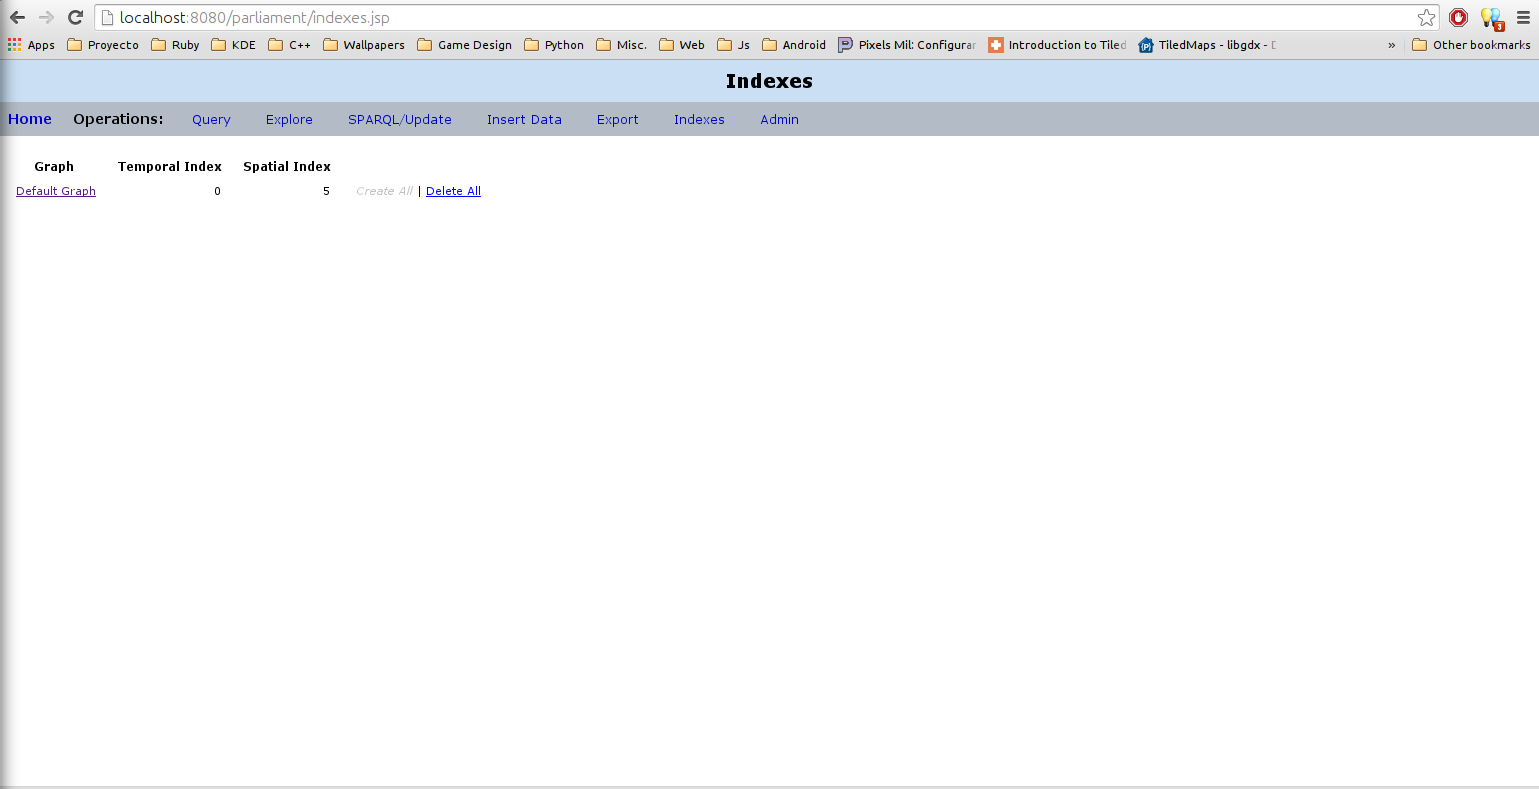
\includegraphics[width=.8\textwidth]{fig/parliament}
  \caption{Web interface of the parliament triple store}
  \captionsetup{font={footnotesize,bf,it}}
  \label{fig:parliament}
\end{figure} 

\subsection{Database connector}

After installing the database, the next step is to develop the database connector. This connector is used to programatically send queries to the data store. Three types of queries will be sent to the endpoint, accessible through the URL \texttt{http:localhost:8080/parliament/sparql}:

\begin{description}
\item[Select] Used to retrieve data from the database. Select queries need to specify a series of bindings, variables that will be retrieved from the database; and a \textit{where} clause which will contain the information actual query. The structure followed is shown on listing \ref{lst:sparql-select}

\begin{listing}[ht]\centering
  \begin{minipage}{.6\textwidth}
    \begin{minted}[linenos=true,mathescape,gobble=6]{text}
	     SELECT ?s ?p ?o #variables to be bound separated by a whitespace
	     WHERE {
	       ?s ?p ?o . 
	     }
    \end{minted}
  \end{minipage}
  \caption{SPARQL Select structure}\label{lst:sparql-select}
\end{listing}

\item[Modify] Used to insert or delete data from the database or both at the same time. SPARQL does not allow to modify existing data, however, it is possible to delete old data and insert the new version in the same query. In order to just insert or delete data, the corresponding part on these queries is omitted. The of the queries is shown in listing \ref{lst:sparql-modify}:

\begin{listing}[ht]\centering
  \begin{minipage}{.6\textwidth}
    \begin{minted}[linenos=true,mathescape,gobble=6]{text}
	     MODIFY
	     DELETE {
	       ?s foaf:name ?name . 
	     }
	     INSERT {
	       ?s foaf:name "new name" . 
	     }
	     WHERE {
	       ?s foaf:name ?name . 
	     }
    \end{minted}
  \end{minipage}
  \caption{SPARQL Modify structure}\label{lst:sparql-modify}
\end{listing}
 
\item[Ask] \textit{Ask} queries are used to check if a set of triples exist in the data store or not. They are identical to \textit{Select} queries, however, they just return a boolean value. In this platform they are used to check the uniqueness of resources. The structure of these queries is shown in listing \ref{lst:sparql-ask}:

\begin{listing}[ht]\centering
  \begin{minipage}{.6\textwidth}
    \begin{minted}[linenos=true,mathescape,gobble=6]{text}
	     ASK { ?s ?p ?o }
    \end{minted}
  \end{minipage}
  \caption{SPARQL Modify structure}\label{lst:sparql-ask}
\end{listing}
\end{description}

\subsubsection*{Intermediate Objects}

The controller uses a SPARQL client to communicate with the database, however, before the actual query is sent to the database, it has to be built by the application. The \textit{query maker} that is used by the rest of the application uses a factory to build objects which represent those queries. Then the client will transform these objects into query strings that can be sent to the application.

The reason to use objects instead of directly writing the query is for convenience. It is easier to handle a JavaScript object in the application that a plain string, thus, the server can objects until the moment to send the query through HTTP is reached. These objects are defined in the \textit{connector\_object.js} file, whose contents are shown in listing \ref{lst:sparql-objects}.

\begin{listing}[ht]\centering
  \begin{minipage}{.6\textwidth}
    \begin{minted}[linenos=true,mathescape,gobble=6]{js}
	     function ModifyQuery(del, insert, where){
	       if(del)
	         this.del = del;
	       if(insert)
	         this.insert = insert;
	       if(where)
	         this.where = where;
	     }
	     module.exports.ModifyQuery = ModifyQuery;
	     
	     function ModifyQuery(bindings, where, others){
	     	if(bindings)
	     	  this.bindings = bindings;
	     	if(where)
	     	  this.where = where;
	     	if(others)
	     	  this.others = others;
	     	}
	     module.exports.SelectQuery = SelectQuery;
    \end{minted}
  \end{minipage}
  \caption{The definition of the connector objects}\label{lst:sparql-objects}
\end{listing}

\subsubsection*{Query factory}

The query factory is the class that creates the intermediate objects which will be transformed into the final queries. The implementation of the factory is divided into four classes; the main class containing the methods for creating the general queries and retrieving notes and other three classes containing the methods for creating the query objects that retrieve the defined models from the database.

A good amount of functions has been defined in this cases, one for each possible request and even several for the same request. One example of this methods is shown on listing \ref{lst:factory}, which is used to insert a user in the data store.

\begin{listing}[ht]\centering
  \begin{minipage}{.8\textwidth}
    \begin{minted}[linenos=true,mathescape,gobble=6]{js}
	       this.new = function(args){ 
	         var userid = calculateURI('user', args.name);
	         var avatar = calculateURI('user', args.name, 'foaf_depiction', 'avatar');
	     
	         var where = 'BIND (' + userid + ' AS ?s) . BIND (' + avatar + ' AS ?avatar)';
	         var insert = '?s rdf:label "' + args.name + '" . \
	         ?s rdf:type foaf:Person . \
	         ?s foaf:nick "' + args.name + '" . \
	         ?s foaf:mbox "' + args.email + '" . \
	         ?s foaf:depiction ?avatar . \
	         ?avatar rdf:type sorelcom:Image . \
	         ?avatar sorelcom:storedOn "/images/icon/user.png" . ';
	     
	         return new ModifyQuery(null, insert, where);
	       };
    \end{minted}
  \end{minipage}
  \caption{A query factory method}\label{lst:factory}
\end{listing}

\subsubsection*{SPARQL client}

The SPARQL client is just a regular HTTP client that uses a series of templates to transform the objects created by the factory into actual SPARQL queries. In order to create a SPARQL client, a endpoint to which queries will be thrown and the prefixes that will be perpended to these queries are specified.

This approach allows to use the client on any endpoint, even if it is not part of the system. An example of the query transformation done by the client can be found in listing \ref{lst:transformation}, where a object and the corresponding SPARQL query are shown.

\begin{listing}[ht]\centering
  \begin{minipage}{.6\textwidth}
    \begin{minted}[linenos=true,mathescape,gobble=6]{js}
	       /** Before the transformation process */
	       var query object = {
	         bindings: '?name ?email'
	         where: '?s a foaf:Person . \
	           ?s foaf:name ?name . \
	           ?s foaf:email ?email .';
	         other: 'LIMIT 5' 
	       };
	       /** After the transformation process */
	       var query =
	         'PREFIX foaf: <http://xmlns.com/foaf/spec/> \
	         SELECT ?name ?email \
	         WHERE { \
	           ?s a foaf:Person . \
	           ?s foaf:name ?name . \
	           ?s foaf:email ?email . \
	         } LIMIT 5';
    \end{minted}
  \end{minipage}
  \caption{Query object to SPARQL transformation}\label{lst:transformation}
\end{listing}

In addition to sending requests to the endpoint, the client also has the task of transforming the response of the database into JSON objects to be sent to the requester. The responses of the database is a JSON file following the specification for serializing SPARQL responses as JSON \cite{sparql-json}, the client just takes that serialization and transforms it into a JSON manageable by the application or into a GeoJSON. An example of this transformation is shown in listing \ref{lst:geojsontransform}

\begin{listing}[ht]\centering
  \begin{minipage}{.85\textwidth}
    \begin{minted}[linenos=true,mathescape,gobble=6]{json}
 
	       {
	         "head": { "vars": [ "name" , "geometry" ]
	         } ,
	         "results": { 
	           "bindings": [
	             {
	               "name": { "type": "literal" , "value": "Example feature" } ,
	               "geometry": { 
	                 "type": "literal" , 
	                 "value": "POINT(0 0)", 
	                 "datatype": "http://www.opengis.net/ont/geosparql#wktLiteral" 
	               }
	             } 
	           ]
	         }
	       }

	       {
	         "type": "Feature",
	         "geometry": {
	           "type": "Point"
	           "coordinates": [0, 0]
	         }
	         "properties": {
	           "name": "Example feature"
	         }
	       }
    \end{minted}
  \end{minipage}
  \caption{RDF-JSON to GeoJSON transformation}\label{lst:geojsontransform}
\end{listing}

\subsubsection*{GeoSPARQL}

The usage of GeoSPARQL on the connector is essential in order to be able to implement some of the functions of the API. One example of this is a function that obtains all the geographical features inside a given bounding box, a typical function in GIS platforms.

In order to do this, special SPARQL queries, which make use of GeoSPARQL implicit relations and functions have to be used. Listing \ref{lst:within} shows the implementation of the query for the aforementioned use case.

\begin{listing}[ht]\centering
  \begin{minipage}{.85\textwidth}
    \begin{minted}[linenos=true,mathescape,gobble=6]{text}
      SELECT ?name ?description ?geometry ?category ?difficulty WHERE
      {
        ?geom geo:sfIntersects 
          [ a geo:Geometry; 
            geo:asWKT "#bound box#"^^geo:wktLiteral ] . 
        ?s geo:hasGeometry ?geom . 
        ?geom geo:asWKT ?geometry . 
        ?s sorelcom:name ?name . 
        ?s sorelcom:description ?description . 
        OPTIONAL { ?s sorelcom:category ?category } . 
        OPTIONAL { ?s sorelcom:difficulty ?difficulty } . 
      }
    \end{minted}
  \end{minipage}
  \caption{GeoSPARQL "within" query}\label{lst:within}
\end{listing}


\subsection{Geography Utilities}

Located in the \textit{util} folder, the geography utilities module provides functionality to analyze features in GeoJSON format, as well as transforming them to WKT in order to store them in RDF.

Most of this analysis consists in obtaining from a set of coordinates parameters such as maximum and minimum height, ascending distance, descending distance or total distance. A method to calculate the distance between two coordinates has been programmed. This method uses a mathematical formula called the \textit{haversine} formula, which can be found on listing \ref{lst:haversine}.

\begin{listing}[ht]\centering
  \begin{minipage}{.9\textwidth}
    \begin{minted}[linenos=true,mathescape,gobble=6]{js}
         function haversine(pt1, pt2){
           var lon1 = pt1[0],
             lat1 = pt1[1],
             lon2 = pt2[0],
             lat2 = pt2[1],
             dLat = numberToRadius(lat2 - lat1),
             dLon = numberToRadius(lon2 - lon1),
             a = Math.pow(Math.sin(dLat/2), 2) + Math.cos(numberToRadius(lat1)) *
             Math.cos(numberToRadius(lat2)) * Math.pow(Math.sin(dLon/2), 2),
             c = 2 * Math.atan2(Math.sqrt(a), Math.sqrt(1 - a));
           return (6371 * c) * 1000;
         }
    \end{minted}
  \end{minipage}
  \caption{JavaScript implementation of the haversine formula}\label{lst:haversine}
\end{listing}

\subsubsection*{Difficulty score}

The difficulty score of a trail is the most relevant data that can be obtained. This difficulty score not only gives an estimation of how hard can it be to a user to follow a route, it can also be used as a deciding factor when trail recommendations have to be done.

In the current iteration of the algorithm, the difficulty score is just based on the slopes on the trail. This value, which ranges from 0 to 100, is calculated by evaluating the different slopes of a trail, grouping them by steepness and comparing the length of each steepness level to the total distance of the trail.

The implementation of this method is shown on listing \ref{lst:score}.

\begin{listing}[ht]\centering
  \begin{minipage}{.7\textwidth}
    \begin{minted}[linenos=true,mathescape,gobble=6]{js}
      var score = 0;
      var meterValue = maxDifficulty/distance;
      for(var i = 0; i < maxSteep; i++){
        var steepValue = k / (maxSteep-1);
        steepValue = ((1 - steepValue) + 1) * steepValue;
        score += steepValue * meterValue * slopes[i];
      }
      return Math.round(score);
    \end{minted}
  \end{minipage}
  \caption{Score calculation algorithm}\label{lst:score}
\end{listing}

This implementation will first calculate a value dividing the maximum difficulty, 100, by the total distance of the trail. This can be seen as the score value for each meter of the trail.

After this, it will start iterating every integer from 0 to the maximum slope calculated, usually 20\%. A proportion for that steep is calculated, in a way that the highest steep gets a bigger value. This value differs more between steep levels the lower the steepness of the levels, that is, the difference between the 0\% slope and the 1\% slope values is greater than the difference between the 19\% slope and the 20\% slope. This allows to differentiate more between trails with low steepness values, which are the most common.

Finally, the distance traversed in that steepness level, multiplied by the proportion of the steepness and the value for each meter, is added to the score. This way, a value that ranges between 0 and a 100 is obtained, being 0 the value of a trail with no slope and 100 the value of a trail with a constant slope of 20\% steepness.

The route calculation could take more parameters into account, such as the type of terrain , however that is left for future versions of the system.

Some factors, however, cannot be added so easily. The most notable of them is the distance. Distance is usually considered a major factor when evaluating how difficult a route is, however, in this case it presents several problems. 

First, distance can vary a lot, one can find trails that cover solely 500m and others that are as long as 100km. Due to this, it is difficult to limit the range of scores when distance is taken as a parameter. Besides, the actual value of the distance is a very subjective factor. For a person that is traversing the trail by foot it may not count as much as for another person that is running through it. Due to this, it has been decided to leave distance outside of the parameters that affect difficulty.

\subsection{Controllers}

The implementation of the controllers is the most trivial task on the development of the server. The job of the controllers is to take the data received on the request, usually a parameter on the URL or an object on the body of the request, extract the data and call a function of the query maker.

Some functions, usually the ones which insert features to the database, need to be analyzed in order to extract the spatial information implicit on their coordinates. In this cases, the controller routes the information to the \texttt{GeographyUtils} class, receives the information and sends it to the database. Figure \ref{fig:controller-sequence} shows a usual control flow for a controller.

\begin{figure}[ht]
  \centering
  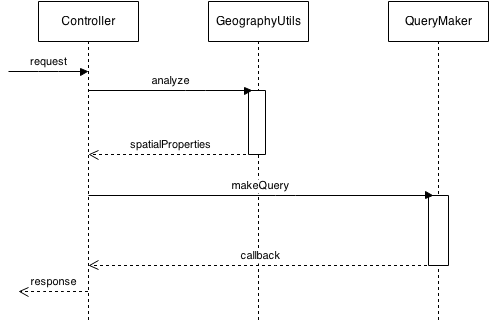
\includegraphics[width=.7\textwidth]{fig/controller-sequence}
  \caption{Sequence diagram for most controller requests}
  \captionsetup{font={footnotesize,bf,it}}
  \label{fig:controller-sequence}
\end{figure} 

Controllers also need to take care of analyzing the response. The Express framework middleware parses the HTTP requests into a JSON object and passes it as a parameter to the controller. In addition, a \textit{response} object is provided to the controller which can be used to send a response. An example is shown in listing \ref{lst:controller}.

\begin{listing}[ht]\centering
  \begin{minipage}{.85\textwidth}
    \begin{minted}[linenos=true,mathescape,gobble=6]{js}
           module.exports.addImage = function(req, res, next){
             if(!req.user)
               return res.send(401);
             
             if(req.body.flowChunkNumber !== req.body.flowTotalChunks)
               return res.send(200); 
               
             short.saveImage(req.files.file, function(err, name){
               if(err) return res.send(500);
               q.Poi.addImage(req.params.id, req.user.name, name, 
                 function(err, data){
                 short.returnOK(err, data, res);
               });
             });
           };
    \end{minted}
  \end{minipage}
  \caption{Controller method for obtaining the trails of a user}\label{lst:controller}
\end{listing}

\subsubsection*{File upload}

Listing \ref{lst:controller} is an example of a controller method that can handle file uploads. Files are uploaded using the \textit{flowjs} \cite{flowjs} library, which sends the files on chunks to the server. 

It is only possible to read the file once all the chunks have arrived. Due to this, it is necessary for the controllers which upload images or videos to the file to check if the chunk of data is actually the last chunk to be sent. In case it is not, then a response acknowledging the client that the data has been received must be sent.

Once the file is fully uploaded, it can be accessed through the \texttt{req.files.file} object. As a sidenote, it is impossible to send more than one file in the same request using this method, however, on the client side it is possible to send multiple files but they will have to be processed one by one on the server.

\subsection{Routes}

The routes of the server are crucial to implement the REST API. In order to define the routes that will be parsed by the server, the Express object offered by the framework must be used. This object exposes five methods to define the URLs that will be read: \textit{get}, \textit{post}, \textit{put}, \textit{delete} and \textit{all}; each of them corresponding to a HTTP method, except for \textit{all} which accepts all methods.

These methods receive two parameters, the first of them is a string or a JavaScript regular expression defining the URL that can be requested and the second argument is the function that is called when a request to that URL is sent.

Listing \ref{lst:routes} defines the URLs from the trail resource of the API. Some of these receive parameters, by specifying a name after a colon; this parameter will be read by the controller on the request object. The same URL can be called from different HTTP operations, however, if no callback is defined for a certain method, the server will send a 404 response.

\begin{listing}[ht]\centering
  \begin{minipage}{.7\textwidth}
    \begin{minted}[linenos=true,mathescape,gobble=6]{js}
           app.get('/api/trails', trails.getList);
           app.post('/api/trails', trails.new);
           app.get('/api/trails/:id', trails.get);
           app.post('/api/trails/:id/images', trails.addImage);
           app.get('/api/trails/:id/images', trails.getImages);
           app.post('/api/trails/:id/post', trails.addPost);
           app.get('/api/trails/:id/post', trails.getPosts);
    \end{minted}
  \end{minipage}
  \caption{API implementation for the trails resource}\label{lst:routes}
\end{listing}

\subsection{Recommendations}

Recommendations, which are currently shown on the profile page of a user, are obtained using SPARQL queries. It is possible to do so thanks to the level of complexity that can be embedded into a single query.

In the first version of the recommendations implemented, the following factors are taken into account:

\begin{itemize}
\item Score of trails
\item Routes traversed by buddies
\item Routes traversed by followed persons
\item Routes added by buddies
\item Routes traversed by followers
\item Distance of the route to the usual location of the user
\end{itemize} 

Listing \ref{lst:recommendation} shows some criteria used on queries to obtain recommendation candidates. It is noteworthy mentioning that these queries are not done independently, they are merged into a single query; in this document they are shown separately for clarity. 

In addition to the filtering shown, the distance of the routes to the usual location of the user is calculated. This is not an actual filtering factor, however, it server to order the candidate routes by their distance to the user. Once this ordering is done, only the few firsts are picked and sent to the user as actual recommendations. 

\begin{listing}[ht]\centering
  \begin{minipage}{.8\textwidth}
    \begin{minted}[linenos=true,mathescape,gobble=6]{text}
      SELECT DISTINCT ?trail WHERE {
        {
         ?trail a sorelcom:Trail ;
         sorelcom:difficulty ?difficulty .
         FILTER(abs(?difficulty-50) < 25)
       } UNION {
         ?user rdf:label "username"; sorelcom:trailBuddyOf ?buddy .
         ?buddy sorelcom:traversed ?trail .
       } UNION {
         ?user rdf:label "username"; sorelcom:follows ?followed .
         ?followed sorelcom:maker ?trail .
         ?trail a sorelcom:Trail .
       }
       ?trail geo:hasGeometry ?tg .
       ?tg geo:asWKT ?twkt .
       BIND(geof:distance(?tg, 
              "POINT(0 0)"^^geo:wktLiteral, 
              units:metre) 
            AS ?distance)
     }
    \end{minted}
  \end{minipage}
  \caption{Criteria for route recommendations in SPARQL queries}\label{lst:recommendation}
\end{listing}

By following this method, the recommendation system can analyse the existing relationships between users. In addition to this, the location of the user is taken into account to a certain point, recommending only nearby routes when there are sufficient candidates. This way, the expressiveness of RDF is combined with spatial queries in order to build a location aware recommendation service.

Usually, recommendation systems use some sort of artificial intelligence, however due to time constraints it has been impossible to implement a more complex recommendation methods. The only possible AI used is the inference engine of the database. Note however, that this is a first version of the final system and there are plans to improve this recommender system with better algorithms and with the addition of more parameters, such as user reviews.

\subsection{Authentication}

The generator used provides a already built authentication service. This service uses the \textit{passport} and \textit{mongoose} NodeJS modules to provide a way of authenticating and storing users.

\textit{Mongoose} is a object database mapper (ODM) that provides a way of modeling models to be used on mongodb databases. It provides a schema based solution for modeling the application data of NodeJS applications.

\textit{Passport} is a flexible authentication middleware for NodeJS. It is based on the concept of \textit{strategy}, which is a way of representing how the users will be authenticated. Different strategies allow using Facebook or Twitter as authentication services, however, in this project only the local strategy based on local database authentication is used.

The generator used provides a \textit{User} modules (in the \textit{models} folder) which contains a nick name, a email and a password. In addition, it comes with a pre built controller for managing users and authenticating them.

In order to take advantage of this, the project uses the provided model and controllers and builds methods for saving and retrieving from the semantic storage on top of them. An example of this is the creation of users, which follows the following procedure:

\begin{enumerate}
\item Retrieve data from the user and save it to the mongodb database
\item Check that the data has been correctly saved
\item Save the user to the triple store
\item Check that the user has been correctly saved
\item If the user is not correctly saved on the triple store, delete it from the mongodb database
\item Return a response according to the result of the operation
\end{enumerate}

\subsection{Real time communication}

The real time communication to be provided has not been implemented in the first phase of the server development. Instead, in order to be able to provide an early prototype of the web application, this functionality has been delayed until it is needed on the development of the mobile application. 

\section{Development of the web application}\label{sec:webappdev}

\subsection{Angular application structure}

The \textit{app} folder of the project contains the code for the web application. It follows a standard Angular folder structure, consisting on the following:

\begin{description}
\item[bower\_components] Third party libraries installed through bower
\item[styles] Style sheets of the application
\item[scripts] JavaScript code of the project
  \begin{description}
  \item[Controllers] Controller source code
  \item[Services] Service source code
  \item[app.js] Application configuration source code 
  \end{description}
\item[vendor] Third party libraries used
\item[views] HTML views of the application
\end{description}

\subsection{Application}

The application file is the first thing to define in a AngularJS project. It is used to create the application itself, to specify which external modules will be used and which will be the routes and views it accepts.

In order to create single page applications, the framework uses the concept of views. When a Angular application is loaded in a browser, its \textit{index.html} file is shown, however, this document usually has a \textit{view} component defined by the \texttt{ng-view} angular directive.

The router of the framework uses the current URL of the browser to embed a different HTML document, called partial view, in the place where the view should be. In this project, the module \textit{ui-router}, an extension of the regular routes has been used.

This module offers enhanced routing capabilities, such as defining nested views. In order to configure this component, the concept of state is used. A state of the application has a URL and a partial view associated. In addition, a controller can be defined to manage that partial view. Some states however, are abstract, meaning that they are only intermediate states with no specific controller and are used to route to nested views. Listing \ref{lst:app} shows the contents of the \textit{app.js} file of the project. Only two state definitions are shown for clarity purposes, since the real number of states is way bigger. 

First, an application is created using the \texttt{angular.module} function, which receive a name for the application and an array with the names of the modules to use. All the source files, even the modules, are included as regular JavaScript scripts in the \textit{index.html} file and the framework will wait for the full loading of the document to execute the code.

Then, a configuration function is used to specify the states that the application will accept. It is also possible to indicate where the browser should be routed when a URL that does not match any state is introduced.

\begin{listing}[ht]\centering
  \begin{minipage}{.85\textwidth}
    \begin{minted}[linenos=true,mathescape,gobble=6]{js}
         var app = angular.module('sorelcomApp', [
           'ngCookies',
           'ngResource',
           'ngSanitize',
           'ngAnimate',
           'ui.bootstrap',
           'ui.validate',
           'ui.router',
           'ui.router.util',
           'leaflet-directive',
           'flow',
           'restangular',
         ]);
          
         app.config(function ($stateProvider, $urlRouterProvider) {
          
          $stateProvider.state('web', {
            abstract: true,
            url: '',
            templateUrl: 'partials/layout.html'
          });
          $stateProvider.state('web.signup', {
            url: '/signup',
            templateUrl: 'partials/signup.html',
            controller: 'SignupCtrl'
           });
         };
    \end{minted}
  \end{minipage}
  \caption{AngularJS application configuration}\label{lst:app}
\end{listing}

\subsection{API}

The API component is used by the rest of the application almost everywhere, thus it is necessary to build it the first. The API acts as a service which comes uses a module called \textit{Restangular} to query the server.

The service offers a object to the rest of components that can be used to retrieve any resource from the API, in addition to some utility functions. The usage of this object, as well as its definition can be found in listing \ref{lst:api}

\begin{listing}[ht]\centering
  \begin{minipage}{.85\textwidth}
    \begin{minted}[linenos=true,mathescape,gobble=6]{js}
          angular.module('sorelcomApp')
            .service('API', function Geo(Restangular) {
            	this.api = Restangular.all('api');
            	
            	this.getTrail = function(id){
            	  return new Trail(this.api.all('trails').one(id))
            	};
            });
    \end{minted}
  \end{minipage}
  \caption{API service class}\label{lst:api}
\end{listing}

This API uses the concept of remote object to provide a means of receiving data from the server without the need of defining a callback each time the API is called. This objects are just containers for data, initially empty. The objects are created by receiving Restangular object which they call immediately after their creation.

A callback is registered to populate the object when the server responds. This callback will call the \texttt{digest} method of the AngularJS root scope, which causes the application to modify the views in order to show the new data.

In addition, a method is provided so that another callback can be registered for when the data arrives to perform additional operations. If the data has already arrived, the callback will be invoked immediately.

Functions of the data, such as getting points of interest and trails can be executed immediately, for they don't depend on the data to be retrieved from the server, only on the provided id.

Listing \ref{lst:remoteobject} shows the implementation of one of such objects.

\begin{listing}[ht]\centering
  \begin{minipage}{.85\textwidth}
    \begin{minted}[linenos=true,mathescape,gobble=6]{js}
          function User(remote){
            var that = this;
            this.prototype = new RemoteObject(remote);
            
            this.remote.get.then(function success(data){
              that.name = data.name;
              that.firstName = data.firstName;
              that.familyName = data.familyName;
              that.homepage = data.homepage;
              that.about = data.about;
              that.ready = true;
              $rootScope.$digest();
            });
            
            this.getTrails = function(callback){
              this.remote.all('trails').getList(callback);
            };
            
          }
    \end{minted}
  \end{minipage}
  \caption{Remote User class}\label{lst:remoteobject}
\end{listing}

\subsection{Accounts}

Most functions of the accounts component are already provided in the application in a similar manner to the server. The \texttt{Auth} and \texttt{Session} services are already created, however, a few changes have been made to the first of them in order to include the functionality needed to require login on some functions.

In addition, the sign up controller and view are provided, and have been left almost unchanged. This controller allows to register a user using a nick name, a email and a password. The only change made has been introducing a double password check before sending the data to the server.

The profile on the other hand is not created during the scaffolding. The profile controller simply downloads the information of the current logged user, using a convenience method of the user resource on the API. This information is displayed in a simple manner in the view and a form is provided to modify it.

When a user signs up it will be immediately redirected to the profile page, in order for it to update the data of his account, such as names and profile picture. It is also possible to see al the activity that the user has done on the platform through this page. Of course, the access is restricted in a way that each user may only access his own profile.

The profile is also used to show recommendations for the user, however, it is not the only place where these can be viewed. If a person is logged in and goes to the homepage, it will be able to see the five trails that are considered most fitting.

\subsection{Web}

The component that has been called "Web" due to its similarity to that of a regular web page consists on four pieces, the home page, the search page and the feature and user views.

\subsubsection*{Home page}

The home page consists on a simple controller that downloads the latest activity on the platform or the user recommendations if the user is signed in. The results are displayed on the page using a peculiar slider.

Since the home page is the first view where a user will arrive when entering the platform, it is important that it is visually appealing. Due to this, the information obtained from the server is not displayed \textit{as is}. 

Since this information will always consist on geographical features which have been created or modified recently, the view shows them on a map. A slider is created which will allow the user to see different maps containing the features obtained. The interaction of these maps has been disabled so that there is no interference with the interaction with the slider. In addition, a event checks when the slide has changed in order to recalculate the size of the map, necessary due to the implementation of the Leaflet library.

\subsubsection*{Search page}

The search page offers a simple interface to make text based search on the server. The controller's only task is to send the query string to the server and to wait for the response to arrive.

Most of the work is done on the view. Since the received data is heterogeneous, users, trails or points of interest may be received; the view must take care of showing the different information of any of the results. This is done using angular directives to hide or show HTML elements. The code for this is shown on listing \ref{lst:search-view}.

\begin{listing}[ht]\centering
  \begin{minipage}{.85\textwidth}
    \begin{minted}[linenos=true,mathescape,gobble=6]{html}
      <main>
       <ul>
        <li ng-repeat="item in searchResults" class="row">
         <a ui-sref="{{makeRef(item)}}" class="col-sm-12 col-xs-12">
          <article>
           <div class="icon col-md-2 col-sm-2 col-xs-2">
            <img ng-src="{{makeIconUrl(item)}}" alt="icon">
           </div>
           <div class="info col-md-9 col-sm-10 col-xs-10">
            <h5>{{item.name}}</h5>
            <div class="details">
             <p ng-if="item.content">{{item.content | limitTo: 40 }}...</p>
             <p ng-if="item.comments">
              <span class="fa fa-comment"> {{item.comments || 0}} </span>
             </p>
             <p ng-if="item.author">
              <span class="fa fa-user">&nbsp;</span> 
              {{item.author}} 
             </p>
            </div>
           </div>
          </article>
         </a>
        </li>
       </ul>
      </main>
    \end{minted}
  \end{minipage}
  \caption{The search view document}\label{lst:search-view}
\end{listing}

Several directives have been used in this (and other) views, including the following:

\begin{description}
\item[\texttt{ng-repeat}] Iterates over a array on the scope and creates a element for each instance.
\item[\texttt{ng-if}] Creates a HTML element when the condition is fulfilled and destroys it when not.
\item[\texttt{ui-sref}] Specifies the state to which the link leads. Provided by the \textit{ui-router} module.
\item[ng-src] Alternative to the \texttt{src} directive which admits brackets (used to indicate angular variables).
\item[\texttt{ng-show} and \texttt{ng-hide}] Hides or shows a html element depending on a condition. Similar to \texttt{ng-if} however it does not create or destroy elements. More efficient when there is a high change ratio on the data. Not used on the shown view.
\end{description}

\subsubsection*{Feature page}

The feature page is just a view showing the details of a certain feature, that is, a point of interest or a trail. The page uses a map to provide a representation of the feature.

To create this map, the \textit{Leaflet-angular-directive} module is used, which allows to embed map following an Angular programming style. It is possible to create a map without using this module, however, for maps which provide solely viewing functionality is is way more convenient to use the module. The usage of this directive is shown in listing \ref{lst:leaflet-angular}.

\begin{listing}[ht]\centering
  \begin{minipage}{.4\textwidth}
    \begin{minted}[linenos=true,mathescape,gobble=6]{html}
      <leaflet width="100%" 
        height="300px" 
        geojson="geojson" 
        id="viewMap">
      </leaflet>
    \end{minted}
  \end{minipage}
  \caption{Leaflet usage with angular on feature pages}\label{lst:leaflet-angular}
\end{listing}

Images and videos of a feature are shown on this page on a slider. Reviews are also shown on this view, and the uploading of actual posts is implemented through a form which requires a text and a numerical value for the rating.

The information is displayed in a similar manner to the search page, by using angular directives the information that is available for different resources is filtered.

\subsubsection*{User page}

The user page is almost identical to the feature page. The view on the user page does not show any map, for there is no spatial data. One the other side, a navigation menu is provided to view the trails, points of interest, buddies and followers of a user.

An option is provided to follow and add a user as a buddy when the user being viewed is different from the user logged in. In essence it works in the same way as the feature page, all the data is loaded at the start and if the user makes a write action a query is sent to the server.

\subsection{Map}

The Map uses a single general view. This view in addition contains other two nested views, one used for exploring functionalities and the other one offering editing operations.

The general or parent view contains a map which takes the full browser screen. In addition, a sidebar containing the HTML for the nested views. The sidebar can be toggled to be displayed, function that has been implemented completely in CSS.

The controller on the parent view implements only the functionality to show and hide the sidebar. All the map creation is done through a service, shown on listing \ref{lst:map-service}

\begin{listing}[ht]\centering
  \begin{minipage}{.75\textwidth}
    \begin{minted}[linenos=true,mathescape,gobble=6]{js}
     angular.module('sorelcomApp').service('Map', function Map(API){
       var that = this;
       this.initMap = function(id){
         var baseLayers = {
           'OpenStreetMap': L.tileLayer(
             'http://{s}.tile.openstreetmap.org/{z}/{x}/{y}.png',
            )
         };
         this.map = L.map(id, {
           layers: [baseLayers.OpenStreetMap],
           minZoom: 3,
           worldCopyJump: true
         });
         L.control.layers(baseLayers, null, {position: 'topleft'})
           .addTo(this.map);
         this.map.locate({ setView: true, maxZoom: 15 });
       };
     });
    \end{minted}
  \end{minipage}
  \caption{Map service implementation}\label{lst:map-service}
\end{listing}

This service is used by the rest of the explorer and controller services to access the map object and add or manipulate data on it. The controllers on the map component are just gateways that call the methods defined on the services from the views, the actual computation is done on the services. 

\subsubsection*{Explorer}

The explorer does offers a single function. This function is called every time the map is moved or zoomed and queries the server for the features that can be found on the current viewport of the map, represented by its bounding box.

The explorer also generates HTML elements that will be bound to every feature shown in the map. This is used to show the text data (name, description) of a element and to link to the corresponding feature page.

The basic functions of the explorer are shown in listing \ref{lst:explorer}. The \texttt{loadGeoJSON} function takes the results and parses them to create the layers and the popups that will be added to the map.

Trails are only shown when the zoom level is enough to distinguish the routes from points. This is determines by the \texttt{canViewRoutes} function, which check the zoom level of the map. If it is not enough, then the server is asked to return only points of interest.

\begin{listing}[ht]\centering
  \begin{minipage}{.85\textwidth}
    \begin{minted}[linenos=true,mathescape,gobble=6]{js}
      angular.module('sorelcomApp')
       .service('Explorer', function Explorer($rootScope, $q, API, Map, $compile){
    
        this.init = function(){
          Map.map.on('moveend', showView);
        };
    
        function showView(geojson){
          if(!that.categories)
            return;
          var query = { bbox: Map.map.getBounds().toBBoxString() }
          if(!canViewRoutes())
            query.type = 'POI';
     
          that.canceler = $q.defer();
     
          API.withHttpConfig({timeout: that.canceler}).get('within', query).then(
            loadGeoJSON);
        }
      });
    \end{minted}
  \end{minipage}
  \caption{Explorer service implementation}\label{lst:explorer}
\end{listing}

The explorer provides no direct interaction with the user, except for the map zooming and moving event. Instead, the space available on the sidebar is used to show links to the detailed views of each feature and to show a legend of the icons used to represent each element on the map.

\subsubsection*{Editor}

The editor provides several functions related to the manipulation of trails and points of interest.

\begin{description}
\item[Uploading of a GPX file] The upload of GPX files is independent of the map, however, it is accessible in this component because all functions that upload data are grouped on it.

The upload opens a modal which will load a GPX file specified by the user. This GPX is converted to a GeoJSON object to be manipulated by the application and the different features are extracted. Only one can be picked to be created.

Once a feature is picked, a form is used to obtain the relevant data such as the name of the feature or the category if it is a point of interest. This data is sent through a post request to the server.

\item[Drawing a trail] A trail is drawn by adding coordinates to a feature. For this, the editor creates a empty polyline and adds it to a map. After that, a callback is bound to the map click event which adds a coordinate to the polyline. This only happens if the distance between the previous coordinate and the new one is less than 500 meters. The method for doing this is shown on listing \ref{lst:draw}

\begin{listing}[ht]\centering
  \begin{minipage}{.80\textwidth}
    \begin{minted}[linenos=true,mathescape,gobble=6]{js}
      this.startDraw = function(){
          Tooltip.setText('Click on the map to start editing');
          that.editing = L.polyline([]).addTo(Map.map);
          var latlngs = that.editing.getLatLngs();
      
          Map.map.on('click', function(e){
            if(latlngs.length > 0 && 
              e.latlng.distanceTo(latlngs[latlngs.length-1]) > 500) 
              return;
            that.editing.addLatLng(e.latlng);
            that.editing.redraw();
            Tooltip.setText('');
          });
        };
    \end{minted}
  \end{minipage}
  \caption{Map drawing function}\label{lst:draw}
\end{listing}

Stopping the editing of the trail requires only to unbind the click event. One this is done, the editing variable can be transformed into a GeoJSON object and the procedure to follow is the same as when uploading a GPX file.

\item[Marking a point of interest] The process for marking a point of interest is very similar to that of creating a trail. The difference on implementation is that the click callback must be unbound as soon as the click is done. Besides, once the point is marker, the creation dialog is called instantaneously. The implementation of this functionality is shown in listing \ref{lst:mark}.

\begin{listing}[ht]\centering
  \begin{minipage}{.85\textwidth}
    \begin{minted}[linenos=true,mathescape,gobble=6]{js}
      this.markPOI = function(){
        Tooltip.setText('Click on the map to choose location');
        Map.map.on('click', function(e){
          this.stopTask();
          Modal.create(L.marker(e.latlng).toGeoJSON());
        });
      };
    \end{minted}
  \end{minipage}
  \caption{Map point of interest marking function}\label{lst:mark}
\end{listing}

\item[Editing a existing trail] In order to edit a trail, a dialog is prompted to ask the user to import from a GPX file of to download it from the platform. If it is imported from a GPX, the functionality mentioned before is used, however, instread of uploading to the platform, it is shown in the map. If it is downloaded from the platform, a list of trails is obtained using the API and the GeoJSON for one of them is obtained when the user selects it.

In this case the JSON file cannot be directly added into the map. It has to be processed first into a editable polyline, which will be the layer added to the map. This editable polyline is developed as a plugin to the Leaflet library.
\end{description}

\subsubsection*{Editable polyline plugin}

In order to edit trails, a means to do so with a point and click interface is provided through the plugin. The goal is to let the users drag the coordinates of a polyline in order to edit them. The library does not provide any event callback that would allow this in any way, the only draggable elements are markers, which represent single points.

A workaround to providing editable lines is creating a polyline and binding each of its coordinates with a marker that can be dragged. When the marker is dragged, then the coordinates of the line can be updated with the new position. Listing \ref{lst:marker-editable} shows the code for this.

\begin{listing}[ht]\centering
  \begin{minipage}{.7\textwidth}
    \begin{minted}[linenos=true,mathescape,gobble=6]{js}
      this.markerGroup = L.LayerGroup();
      this.markers = [];
      this.latlngs = this.line.getLatLngs();
      for(var i = 0, l = this.latlngs.length; i < l; i++){
        var marker = L.marker(latlngs[i]);
        this.markers.push(marker);
        marker.addTo(this.markerGroup);
        marker.on('dragend', function(e){
          latlngs[markers.indexOf(marker)] = e.latlng;
          line.redraw();
        });
      }
      this.markerGroup.addTo(map);
    \end{minted}
  \end{minipage}
  \caption{Code for adding markers to allow edition of polylines}\label{lst:marker-editable}
\end{listing}

This however does not serve to improve the performance of the editable line. In order to avoid excessive computation time, markers are removed from the map when too many of them are shown at the same time. To do this, a check must be made every time the map is moved or zoomed and if the number of markers is above the maximum, the layer where they are kept is removed. Code for this functionality is shown on listing \ref{lst:marker-check}.

\begin{listing}[ht]\centering
  \begin{minipage}{.75\textwidth}
    \begin{minted}[linenos=true,mathescape,gobble=6]{js}
      var that = this;
      map.on('moveend', function(){
        var count = 0;
        for(var i = 0, l = that.markers.length; i < l; i++){
          if(map.getBound.contains(that.markers[i].getLatLng()){
            count++;
          }
        }
        if(count > maxMarkers && map.hasLayer(that.markerGroup))
          map.removeLayer(that.markerGroup);
        else if(count <= maxMarkers && !map.hasLayer(that.markerGroup))
          map.addLayer(that.markerGroup);
      });
    \end{minted}
  \end{minipage}
  \caption{Code for removing markers to avoid performance issues}\label{lst:marker-check}
\end{listing}

In addition to coordinate dragging, it is necessary to provide functionality to add and remove coordinates from the map. Adding functionality is provided by setting additional markers in the midpoint between each adjacent coordinate pair. When one of these extra markers is dragged, a new coordinate is added to the polyline.

Removing markers on the other hand is simpler. When the user right clicks a marker the corresponding coordinate is removed. This however implies calculating a new midpoint, so that it is still possible to add coordinates in that segment. Pseudo code for these actions are shown on listings \ref{lst:marker-add} and \ref{lst:marker-remove}, the actual code is not shown for clarity purposes.


\begin{listing}[ht]\centering
  \begin{minipage}{.7\textwidth}
    \begin{minted}[linenos=true,mathescape,gobble=6]{js}
      extraMarker.on('dragend', function(e){
        var index = this.extraMarkers.indexOf(e.target) + 1;
        this.latlngs.splice(index, 0, e.latlng);
        this.markerGroup.splice(index, 0, L.marker(e.latlng));
        coordinateAdded(index);
      });
    \end{minted}
  \end{minipage}
  \caption{Add coordinates on a editable line}\label{lst:marker-add}
\end{listing}

\begin{listing}[ht]\centering
  \begin{minipage}{.7\textwidth}
    \begin{minted}[linenos=true,mathescape,gobble=6]{js}
      marker.on('click', function(e){
        var index = this.markers.indexOf(e.target);
        this.latlngs.splice(index, 1);
        coordinateRemoved(index);
      });
    \end{minted}
  \end{minipage}
  \caption{Remove coordinates on a editable line}\label{lst:marker-remove}
\end{listing}

\begin{listing}[ht]\centering
  \begin{minipage}{.7\textwidth}
    \begin{minted}[linenos=true,mathescape,gobble=6]{js}
      function midpoint(latlng1, latlng2){
        return L.latLng((latlng1.lat+latlng2.lat)/2, 
          (latlng1.lng+latlng2.lng)/2);
      };
    \end{minted}
  \end{minipage}
  \caption{Midpoint formula implementation}\label{lst:midpoint}
\end{listing}

The calculation of the middle point of two coordinates is done through the midpoint formula, as shown in listing \ref{lst:midpoint}.

\subsection{Dialogs}

The dialogs component offers means of providing interaction with the user through pop-up boxes, also called modals.

The central class on this component is called the \texttt{Modals} service, used to invoke this dialogs. The \textit{Twitter Boostrap} framework offers functionality and styles to create dialogs and the module \textit{ui-bootstrap} provides Angular services to use them.

This is done through the \textit{\$modal} service, which allows creating a dialog from a defined HTML template and a given controller. The central class of the component uses this service to create different predefined modals. One example of this is shown on listing \ref{lst:modals-shortcut}

\begin{listing}[ht]\centering
  \begin{minipage}{.7\textwidth}
    \begin{minted}[linenos=true,mathescape,gobble=6]{js}
      angular.module('sorelcomApp').service('Modal', function ($modal){
        this.loadGPX = function(){
          var modal = $modal.open({
            templateUrl: 'partials/modals/load.html',
            controller: 'GPXLoadCtrl',
          });
          return modal.result;
        };
      });
      
    \end{minted}
  \end{minipage}
  \caption{Modal invoking shortcuts}\label{lst:modals-shortcut}
\end{listing}

Every method that creates a shortcut returns the \textit{result} of that shortcut. This object is what is denominated a \textit{promise}. Promises are event listeners that listen to a single success of failure from a asynchronous callback. It is possible to define what the promise will do in case of success and what it will do in case of error, in a way similar to callbacks.

By returning the promise object to the controller summoning the modal, it is possible to let it define how the application will behave once the modal finishes its task. This way it is possible to reuse the same code for different functions. For example, the GPX loader modal will return a GeoJSON as a result, which can be used to create a new modal and upload it or can be directly embedded in a map.

The controllers of the modals will return a result using a service called \textit{\$modalInstance} provided by the same Angular module. Using the function \texttt{\$modalInstance.close()} it is possible to return values to whoever is listening the promise. Example \ref{lst:modalinstance} shows how this works.


\begin{listing}[ht]\centering
  \begin{minipage}{.7\textwidth}
    \begin{minted}[linenos=true,mathescape,gobble=6]{js}
      
      $scope.continue = function(){
        $modalInstance.dismiss();
        Modal.create($scope.selected);
      };
      
      $scope.import = function(){
        $modalInstance.close($scope.selected);
      };
      
    \end{minted}
  \end{minipage}
  \caption{Modal closing and communicating functions}\label{lst:modalinstance}
\end{listing}

Most of the implementation of the modals consists in simple functions, mostly to get some data from the user, taken from a form or a button. Most of the implementation of the modals consists on this way of communication, to provide ease of use and reusability.

One modal, however, performs a relatively complex function by itself.

\subsubsection*{GPX loading modal}

The GPX loading modal is in charge of parsing GPX files and extracting the features contained within. In order to do this, a small JavaScript library called \textit{togeojson} is used, which converts from well known geographic encoding formats, such as GPX and KML to a GeoJSON object.

This library will always return a \textit{FeatureCollection} even when only one feature is found. The controller for this modal delegates on a service called \textit{Loader}, which uses this library to generate a GeoJSON and then parses the GeoJSON extracting all of its features.

Once all features are extracted, the user is shown a menu with various maps, each containing one of the features. Once on is selected, the rest of the creation procedure is just standard form data extraction and AJAX calls to the server.

The code for the feature extraction in shown on listing \ref{lst:gpxparse}

\begin{listing}[ht]\centering
  \begin{minipage}{.8\textwidth}
    \begin{minted}[linenos=true,mathescape,gobble=6]{js}
       angular.module('sorelcomApp').service('Loader', function Loader(){
       
        this.extractLayers(text, format) {
          var geojson = toGeoJSON.gpx(jQuery.parseXML(text));
          if(!geojson) return null;
          if(geojson.type === "FeatureCollection"){
            var json = [];
            for(var i = 0, len = geojson.features.length; i < len; i++){
              geojson.features[i].properties.gpx = text;
              json.push(geojson.features[i]);
            }
            return json;
          } else {
            return [geojson];
          }
        }
       });
    \end{minted}
  \end{minipage}
  \caption{Modal closing and communicating functions}\label{lst:gpxparse}
\end{listing}

\section{Development of the Mobile application}

The mobile application reuses many of the classes present on the web application. Thanks to this, the accounts and web components have been reused without any major change. The folder structure of the mobile application is the following:

\begin{description}
\item[app] Contains the application, in a similar way to the server. The contents will be compiled into the \textit{www} folder in order to deploy the application.

\item[www] Contains the scripts, views and styles that the deployed application will use.

\item[test] Contains the tests

\item[platform] Contains the code specific to the platform. In the \textit{src} folder inside is where the Java classes of the application can be found.
\end{description}

The changes for the API have been minimal too, instead of defining a relative URL to make requests to, the URL has been changed to the absolute URL of the server where the application is hosted. The change simply means that instead of having \textit{/api} as the base URL of the API service, this URL will be \textit{apps.morelab.deusto.es/sorelcom/api}.

The functionality offered by the modals has also slightly changed. Since the application will only be executed on the mobile, the dialogs are no longer pop up boxes. This implies slight changes to the views and to the controllers in order to remove the communication functions. However, most of the modals, such as the GPX importing have been removed for there is no need of them in the mobile application.

\subsection{Real time functionality - Server side}

In order for the mobile component to communicate in real time with the server, it is necessary to implement this capability on the web server. This is done using the socket.io library.

It is possible to make Socket.IO application and a Express application work in the same machine and port, however, for this it is necessary to modify the server initialization code, found on the root of the server, in the file \textit{server.js}.

For this it is only needed to require the \textit{socket.io} module and to tell the library object to start listening on the web server, as seen on listing \ref{lst:sioinit}.

\begin{listing}[ht]\centering
  \begin{minipage}{.8\textwidth}
    \begin{minted}[linenos=true,mathescape,gobble=6]{js}
       var io = require('socket.io');
       var express = require('express');
       
       var app = express();
       
       ...
       app.listen(config.port, function () {
         console.log('Express server listening on port %d in %s mode', 
         config.port, app.get('env'));
       });
       var sio = io.listen(app);
       require('./lib/socket/init')(sio);
    \end{minted}
  \end{minipage}
  \caption{Socket.IO server initialization}\label{lst:sioinit}
\end{listing}

The \textit{require} keyword is used after the initialization of the socket in order to define the behavior of the WebSocket once connections arrive. The file specified in the \textit{require} call will be passes the Socket.IO object as a parameter and its code will be executes as in a normal module, with the difference that it will not need to export anything.

\subsubsection{Authentication}

Due to the way the real time functionality works, it is necessary to identify the user using the service. Instead of authenticating the user through the socket, the application uses the session established on the web server. 

In order to do this, there is no need to modify code on the existing web server. A secret key is defined on the configuration files when specifying the behavior of the Express session manager. This secret key, \textit{sorelcom secret} during the development of the project, has to be used to configure Socket.IO authorization mechanisms. The code on listing \ref{lst:socketauth} shows how it has been done.

\begin{listing}[ht]\centering
  \begin{minipage}{.8\textwidth}
    \begin{minted}[linenos=true,mathescape,gobble=6]{js}
       sio.configure(function(){
         sio.set('authorization', passportSocket.authorize({
           key: 'connect.sid',
           secret: 'sorelcom secret', //In lib/config/express
           store: config.sessionStore, //In lib/config/express file
           fail : function(data, accept) { accept(null, false); },
           success: function(data, accept) { accept(null, true); }
         }));
       });
    \end{minted}
  \end{minipage}
  \caption{Socket.IO authorization}\label{lst:socketauth}
\end{listing}

\subsubsection*{Communication protocol}

The communication protocol defined in section \ref{sec:protocol} is implemented mostly on the server. In order to support this protocol, the server uses a subscription mechanism. 

With this mechanism, a connection can subscribe or unsubscribe from a service, such as following a determined trail, at will. This enables to have a undetermined amount of services functioning at the same time, for example, a client may be checking for nearby features and at the same time following trail A and B. Besides, it is relatively easy to implement using JavaScript dictionaries.

When a client connects to the server, a \textit{State} object is created, which will contain the configuration options and the services it is subscribed to. It is noteworthy to mention that the configuration options are global, thus it is not possible to configure trail following distance differently for each trail. The implementation of this class is shown in listing \ref{lst:subscriptions}

\begin{listing}[ht]\centering
  \begin{minipage}{.8\textwidth}
    \begin{minted}[linenos=true,mathescape,gobble=6]{js}
       function State(){
         this.subscriptions = {}
         //Load configuration from the user profile
         this.configs = loadConfiguration(); 
         this.subscribe = function(service){
           if(this.active.service){
             var id = this.subscriptions.service.id;
             this.subscriptions.service = null;
             return id;
           } else {
             this.subscriptions.service = 
               ServiceFactory.createService(service);
             return this.subscriptions.service.id;
           }
         }
         this.setConfig = function(key, value){
           if(this.configs.key)
             this.configs.key = value;
         };
       }
    \end{minted}
  \end{minipage}
  \caption{Subscribing functionality}\label{lst:subscriptions}
\end{listing}

Services follow a pattern similar to regular object oriented interfaces. The idea behind this is to use polymorphism to call the services to which the connection is subscribed. However, JavaScript does not provide support for inheritance out of the box. Still, it is possible to implement polymorphism redefining methods of the prototype of the class. The implementation of the service that implements the trail following service is shown on listing \ref{lst:follow}.

\begin{listing}[ht]\centering
  \begin{minipage}{.8\textwidth}
    \begin{minted}[linenos=true,mathescape,gobble=6]{js}
       function FollowService(trail){
         this.trail = trail;
         this.prototype = new Service('follow ' + trail);
         
         this.prototype.process(coordinates, callback){
           q.isInside(coords, trail, function(err, data){
             if(err) return callback(err);
             if(data.boolean === false) return callback(null, 'FALSE'); 
             q.isLast(trail, function(err, data){
               if(err) return callback(err);
               if(data.boolean === false)
                 return callback(null, 'TRUE');
               callback(null, 'FINISH');
             });
           });
         }
       }
    \end{minted}
  \end{minipage}
  \caption{Trail following service implementation}\label{lst:follow}
\end{listing}

Services implement a function called process, which processes the operations needed to implement the service. The example in listing \ref{lst:follow} queries the database to check if the coordinates are inside of the trail being followed. If they are it checks it the trail has finished. The result is sent through a callback to the main process which will send it as a response to the client.

Due to the way JavaScript works, having a base class in this moment makes no difference with just creating the different services without any inheritance. This approach however, provides a higher extensibility if there is a need to add data to the base class in the future.

The main loop of the socket server implements the functionality needed to read the data. This function checks the command received to perform the different operations. When a subscription is asked it will call the \textit{State} object of the client and subscribe a new service. When coordinates are sent to the server it processes all the services it is subscribed to and sends the responses back to the client.

The data received is a JSON object, thus there is no need to parse the query done by the server, it is already presented as a object to the process. A callback is registered for each command sent by the client and the \textit{argument} members of the data sent are read. The code for the listening process can be found in listing \ref{lst:socket}.

\begin{listing}[ht]\centering
  \begin{minipage}{.8\textwidth}
    \begin{minted}[linenos=true,mathescape,gobble=6]{js}
       sio.on('connection', function(socket){
         var state = new State();
         
         socket.on('nearby', function(){
           var service = state.subscribe('nearby'); 
           socket.emit('OK', service.id);
         });
         socket.on('follow', function(trail){
           var service = state.subscribe('follow ' + trail);
           socket.emit('OK', service.id);
         });
         socket.on('config', function(values){
           for(var key in values){
             state.setConfig(values[key].name, values[key].value);
           }
           socket.emit('OK');
         })
         socket.on('coords', function(coords){
           for(var key in state.subscription){
             var service = state.subscriptions[key];
             service.process([coords.lat, coords.lon], function(err, result){
               if(err) return socket.emit('error', err);
               socket.emit(service.id, result);
             });
           }
         })
       });
    \end{minted}
  \end{minipage}
  \caption{Socket server main process}\label{lst:socket}
\end{listing}

The code subscribes (or unsubscribes) a service on the state of the current connection when the appropriate command is received. When coordinates are received the server loops through all the subscribed services and returns the response when each service is finished processing.

It is important that the server returns the identity of the service every time a new subscription is created or one is deleted. This is used in the client to keep a registry of the services running currently.

There is an additional callback used when the socket is disconnected. It is used to clean all the data accumulated by the user.

\subsection{Real time functionality - Client side}

The client side mobile exclusive functionality are directly related to the real time functionality of the system. This includes tracking nearby features, detecting when the user is deviating from a trail or recording a GPX file.

These functionalities are share something in common: they are continuous and executed during large periods of time. Due to this, it is unreasonable to pretend this functionality to work only when the application is on screen.

In native mobile applications, this kind of batch functions are implemented using service processes. Phonegap, however, does not allow this. Since the applications created using this library are run on a WebView, similar to a browser, JavaScript code can only be executed while the application is open.

There is a workaround for this issue however. Phonegap implements native functionality with something called plugins. These plugins are pieces of native code that can be called from the application itself. Therefore, it is necessary to implement the real time functions of the mobile application as plugins.

This implies coding in Java, the native language for the Android platform. The GPS of the device is acessed natively in this classes to provide the server with the current coordinates of the device, and a Socket.IO Java library is used to communicate this to the server.

Due to this, the application ends up using HTML5 development for interface manipulation and interaction (as well as for the functions borrowed from the web application) and using native code for the background processes.

\subsubsection*{Background service plugin}

Two background services need to be implemented in the application. One of them is used for the recording of coordinates of a trail, the other one for the communication with the server.

The first service is the most straightforward one, it just needs to call the GPS on the device every interval of time. To develop the services, a Phonegap plugin called \textit{Background Service Core Plugin}, found in \href{https://github.com/Red-Folder/bgs-core}, has been used. Through the usage of this plugin, it is possible to develop a Android background service using a simple class structure.

In the Java class representing the service, a \textit{doWork} method has to be written that provides a functionality to be executed at each interval. The interval at which it is executed is specified in the JavaScript code.

In order to use this service with the application, it is necessary to edit the android manifest file. This file presents information about the application to the operating system such as the permissions needed and the services it uses. The lines on listing \ref{lst:manifest} have to be added in order to be able to use the services and the GPS of the device. The services and the permissions are located in different parts of the XML document, however they are put here together for convenience purposes.

\begin{listing}[ht]\centering
  \begin{minipage}{.8\textwidth}
    \begin{minted}[linenos=true,mathescape,gobble=6]{xml}
       <uses-permission android:name="android.permission.ACCESS_FINE_LOCATION" />
       ...
       <service android:name="com.sorelcom.services.TrailRecorder">
          <intent-filter>
             <action android:name="com.sorelcom.services.TrailRecorder" />
          </intent-filter>
       </service>
       <service android:name="com.sorelcom.services.Locator">
          <intent-filter>
             <action android:name="com.sorelcom.services.Locator" />
          </intent-filter>
       </service>
    \end{minted}
  \end{minipage}
  \caption{Android manifest file}\label{lst:manifest}
\end{listing}

The trail recorder service will just pick a point every regular interval of time through the \textit{doWork()} method and will add it to a array, which will be returned to the application as a JSON. This way, once the recording finishes, all the GPX data has been received.

The implementation of this method is shown on listing \ref{lst:recorder}.


\begin{listing}[ht]\centering
  \begin{minipage}{.8\textwidth}
    \begin{minted}[linenos=true,mathescape,gobble=6]{java}
       @Override
       protected JSONObject doWork() {
          Location loc = pointRecorder.getLocation();
          if(loc == null)
            return trail;
          JSONArray coords = new JSONArray();
          coords.put(loc.getLatitude());
          coords.put(loc.getLongitude());
          JSONArray array = trail.getJSONArray( "coordinates");
          array.put(coords);
          return trail;
       }
    \end{minted}
  \end{minipage}
  \caption{Recorder service implementation}\label{lst:recorder}
\end{listing}

The \textit{PointRecorder} appearing in the recorder service is different from the one on the design specified in section \ref{sec:mobileappdesign} on chapter \ref{ch:design}. The one used on the service is just a utility class that encapsulates the functionality of the \textit{LocationManager} class used in android to retrieve the current location of the user. 

This point recorder uses the created services as a android context to gain access to the GPS of the device. The code for creating point recorders is shown on listing \ref{lst:pointrecorder}. Since the GPS device may be temporarily disabled, the location manager records the last location and sends it to the user as a fall-back if there is no GPS.

\begin{listing}[ht]\centering
  \begin{minipage}{.8\textwidth}
    \begin{minted}[linenos=true,mathescape,gobble=6]{java}
       public class PointRecorder{
         LocationManager manager;
         Location lastLocation;
       
         public PointRecorder(Context context){
           manager = (LocationManager) context
               .getSystemService(LOCATION_SERVICE);
         }
         
         public Location getLocation(){
           if(locationManager
               .isProviderEnabled(LocationManager.GPS_PROVIDER)){
             lastLocation = locationManager
                 .getLastKnownLocation(LocationManager.GPS_PROVIDER);    
           }
           return lastLocation;
         }
       }
    \end{minted}
  \end{minipage}
  \caption{Recorder service implementation}\label{lst:pointrecorder}
\end{listing}

The last service to implement is the location tracker service. This service has to communicate with the Socket.IO server, for which a client library is needed. A Java implementation of the Socket.IO library has been used for the creation of this functionality. This library can be found in \href{https://github.com/Gottox/socket.io-java-client}. The service is very similar to the tracker service regarding implementation, however, it uses the \textit{doWork()} and configuration methods to communicate information to a class implementing the protocol on the client side. The code of this class is shown on listing \ref{lst:socketclient}.

\begin{listing}[ht]\centering
  \begin{minipage}{.8\textwidth}
    \begin{minted}[linenos=true,mathescape,gobble=6]{java}
       public class SocketIOClient{
         SocketIO socket;      
         ConnectionStatus status;
        
         public SocketIOClient(){
           socket = new SocketIO("http://apps.morelab.deusto.es/sorelcom");
           ConnectionStatus status = new ConnectionStatus();
         }
         public void start(){
           socket.connect(status.callback);
         }
         public void sendCoordinates(Location loc){
           JSONObject object = new JSONObject();
           object.put("lat", loc.getLatitude());
           object.put("lon", loc.getLongitude());
           socket.emit("coords", object);
         }         
         public void addService(String name){
           status.toggleService(name);
         }
       }
    \end{minted}
  \end{minipage}
  \caption{Socket communication client}\label{lst:socketclient}
\end{listing}

The client implementation works in a identical way to the server. When the user want to subscribe to a new service, the socket subscribes adds it to a list of services. The difference is that instead of having a function encoded to a service, the client services will subscribe a callback to the IOCallback object used on the socket. Note that the services mentioned here are different from the android \textit{Services}.

When a new service is added, the a new callback is subscribed to the socket, as shown in listing \ref{lst:clientservice}.

\begin{listing}[ht]\centering
  \begin{minipage}{.8\textwidth}
    \begin{minted}[linenos=true,mathescape,gobble=6]{java}
       Map<String, IOService> active;
       
       public ConnectionStatus(){
         active = new Map<String, IOService>();
         final ConnectionStatus st = this;
         callback = new IOCallback(){
           @Override
           public void on(String event, IOAcknowledge ack, Object... args) {
              if(st.active.contains(event))
                active.get(event).process(args);
           }
         }
       }
       public toogleSubscription(name){
         if(active.contains(name)){
           active.get(name).destroy();
         } else {
           active.put(name, ServiceFactory.createService(service));
         }
       };
    \end{minted}
  \end{minipage}
  \caption{Service subscriptions and server message reading}\label{lst:clientservice}
\end{listing}


Most of the code of the document is not shown on this section, however, the design specifies how the control flow works among the different classes on figure \ref{fig:plugin-flow} on page \pageref{fig:plugin-flow}.

\subsubsection*{Application-to-service communication}

The interface needs to provide a way to communicate the user with the services in order to access this functionality. This includes allowing a user to start or stop following a trail, activating or deactivating the location tracking process and starting to record a GPX.

This is all done through the AngularJS services specified for the mobile client (see \ref{fig:mobile-diagram} on page \pageref{fig:mobile-diagram}). The services, programmed in the native language, are accessed on the JavaScript code through the use of the Cordova library. The code for creating a service can be found on \ref{lst:makeservice}. This code is called when the Angular service handling the Android service is created.

\begin{listing}[ht]\centering
  \begin{minipage}{.8\textwidth}
    \begin{minted}[linenos=true,mathescape,gobble=6]{js}
       var factory =cordova.require(
        'com.red_folder.phonegap.plugin.backgroundservice.BackgroundService');
       var trailService = factory.create('com.sorelcom.services.TrailRecorder');
    \end{minted}
  \end{minipage}
  \caption{Android service creation from the application}\label{lst:makeservice}
\end{listing}

Once the service is started, the application can access a uniform API to set intervals on which the code of the service will be run and to receive results. For this, the application should register for updates on the service. This will cause the application to receive a JSON object, returned by the doWork() method on the service, every interval of time specified.

In addition, the service can be stopped by disabling it's timer. Once this is done, a JSON object corresponding to the result of the last interval is returned. This is used on the GPX tracker to obtain the finished route once the user decides to stop recording.

In addition, the service can receive configuration options through another method on the API. This configuration methods are used on the Location tracker to enable and disable different services, that is, configuration is changed when the user activates or deactivates the nearby feature discovery or when the user decided to start or stop tracking a service. Initialization of the trail recording service is shown on listing \ref{lst:startservice}.

\begin{listing}[ht]\centering
  \begin{minipage}{.8\textwidth}
    \begin{minted}[linenos=true,mathescape,gobble=6]{js}
       trailService.getStatus(function(status){
         startService(status)
       });
       
       function startService(status) {
          if (status.ServiceRunning) {
             enableTimer(status);
          } else {
             myService.startService(function(data){
               enableTimer(data)
             });
          }
       }
    \end{minted}
  \end{minipage}
  \caption{Trail recording service starting from the application}\label{lst:startservice}
\end{listing}

Once the service is started, it is possible to enable a timer interval. Functions for starting the trail recorder timer and receiving data from the service are shown on listing \ref{lst:starttimer}

\begin{listing}[ht]\centering
  \begin{minipage}{.8\textwidth}
    \begin{minted}[linenos=true,mathescape,gobble=6]{js}
       function enableTimer(status) {
          if (status.TimerEnabled) {
             registerForUpdates(status);
          } else {
             this.trail = [];
             myService.enableTimer(recordInterval, function(data){
               registerForUpdates(data)
             });
          }
       }
       
       function registerForUpdates(status) {
          if (!status.RegisteredForUpdates) {
             myService.registerForUpdates(function(data){
               if(data.latestResult != null){
                 //Push last coordinates to the trail
                 this.trail.push(data.latestResult);
               }
             });
          }
       }
    \end{minted}
  \end{minipage}
  \caption{Trail recording timer start and data reception implementation}\label{lst:starttimer}
\end{listing}

\section{Application functionality}

The implementation of the rest of the application is almost identical to that of the web application. The work necessary is just a few modifications on the views, eliminating the dialog communication functionality from the modal controllers and creating the new controllers to communicate with the plugins.

In addition, the functionality to create a geolocated note must be created. This function however can be done using only Phonegap provided functions. The reason for creating background services is just providing the user with a functionality that persists when the phone is blocked. Since posting a note is done in a single point in time, while the application is on screen, there is no need to create a service for this.

Instead, the Phonegap geolocation plugin is used. This plugin accesses the GPS device and provides a single coordinate set representing the current position of the user, perfect for the note posting functionality. The code to obtain this coordinates is shown on listing \ref{lst:phonegap-location}.

\begin{listing}[ht]\centering
  \begin{minipage}{.8\textwidth}
    \begin{minted}[linenos=true,mathescape,gobble=6]{js}
       navigator.geolocation.getCurrentPosition(function(position){
         note.addPosition(
           position.latitude,  
           position.longitude, 
           position.coords.altitude || 0);
       });
    \end{minted}
  \end{minipage}
  \caption{Location retrieval using Phonegap}\label{lst:phonegap-location}
\end{listing}

Once the location is obtained, the note will just be sent as a GeoJSON to the server through a HTTP POST request to the REST API. This is the only functionality noteworthy on the server (besides the services), the rest is a slight modification of the web application functionality.